\chapter{Evaluation}
As mentioned in the methodology, the evaluation was carried out throughout the development lifecycle allowing improvements at each iteration. This chapter describes how the evaluation of a final prototype was conducted to assess functional and non-functional aspects, as well as the technical evaluations that were performed to ensure the accomplishment of the software quality attributes. 

\section{Technical Evaluation}

\subsection{Automated Tests}

Testing an Android application is particularly challenging because opposed to iOS, many manufacturers are allowed to distribute their own devices that run this operating system. This means that an application should be able to work in many different phones with different screen sizes, resolutions or specific hardware components. There is no gold standard to testing an android application other than trying it out on many distinct devices. This normally is an expensive task, but nowadays emerging services make cloud-based devices available so that developers can connect to them remotely to install and test their applications on demand.

Amazon provides such service in the AWS mobile device farm. \footnote{\url{https://aws.amazon.com/device-farm/}} The application was tested by executing automated tests that explore the interface autonomously to discover how it might react to normal user interaction but also under odd circumstances. Another benefit of this service is that the tests are executed in parallel with a number of devices that are widely used (in this case 15) to encounter errors that might arise from different screen types or hardware components. 

The test starts by uploading a packaged version of the application to the service which is then responsible for installing it in different devices of the farm. If the application is able to respond to all simulated user input and keep working under a defined period of time then the test for that specific device has passed. Two iterations of this test allowed for bugs to be found and interface errors were corrected and optimised. In the first test carried out the application was failing on 5 from 15 devices. The logs of the crash were studied and fixed. A second iteration showed a better outcome, just 1 of the 15 devices failed the test. This resulted in improved compatibility.   

\begin{figure}[H]
\begin{adjustbox}{width=1\textwidth,center=\textwidth}
  \centering
  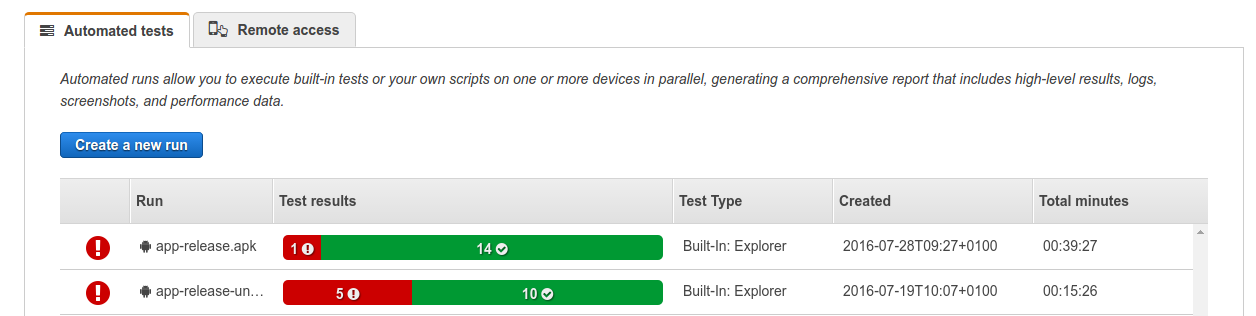
\includegraphics[scale=1]{images/automated_tests.png}
\end{adjustbox}
  \caption[Automated tests on AWS]{Automated tests on AWS}
  \label{fig:automated_tests}
\end{figure}

\subsection{Resources Usage}
To ensure that the application consumes the adequate number of resources off any device, the resource usage of the running application was explored. Android provides tools to monitor the usage of the consumed resources such as battery, bandwidth and memory from any application installed. From its usage the following was identified:
\begin{itemize}
    \item Memory: The application consumes in total 33mb in storage, which is feasible given the modern phones storage capabilities. This storage space was needed in order to provide a better user experience through graphics and animations.
    \item Data usage: Throughout the development process the application was executed several times during almost a month. It used 2.15mb of data in total. This usage is low for an application of this kind.
    \item Battery usage: From using the application on repeated occasions in a dedicated device, it was found that the application doesn't employ any background process. All the communication tasks are performed when the app is open. Also, it does not require the GPS to be on as it will use the location already gathered by the internal phone services.
\end{itemize}


\begin{figure}[H]
\begin{adjustbox}{width=.45\textwidth,center=\textwidth}
  \centering
  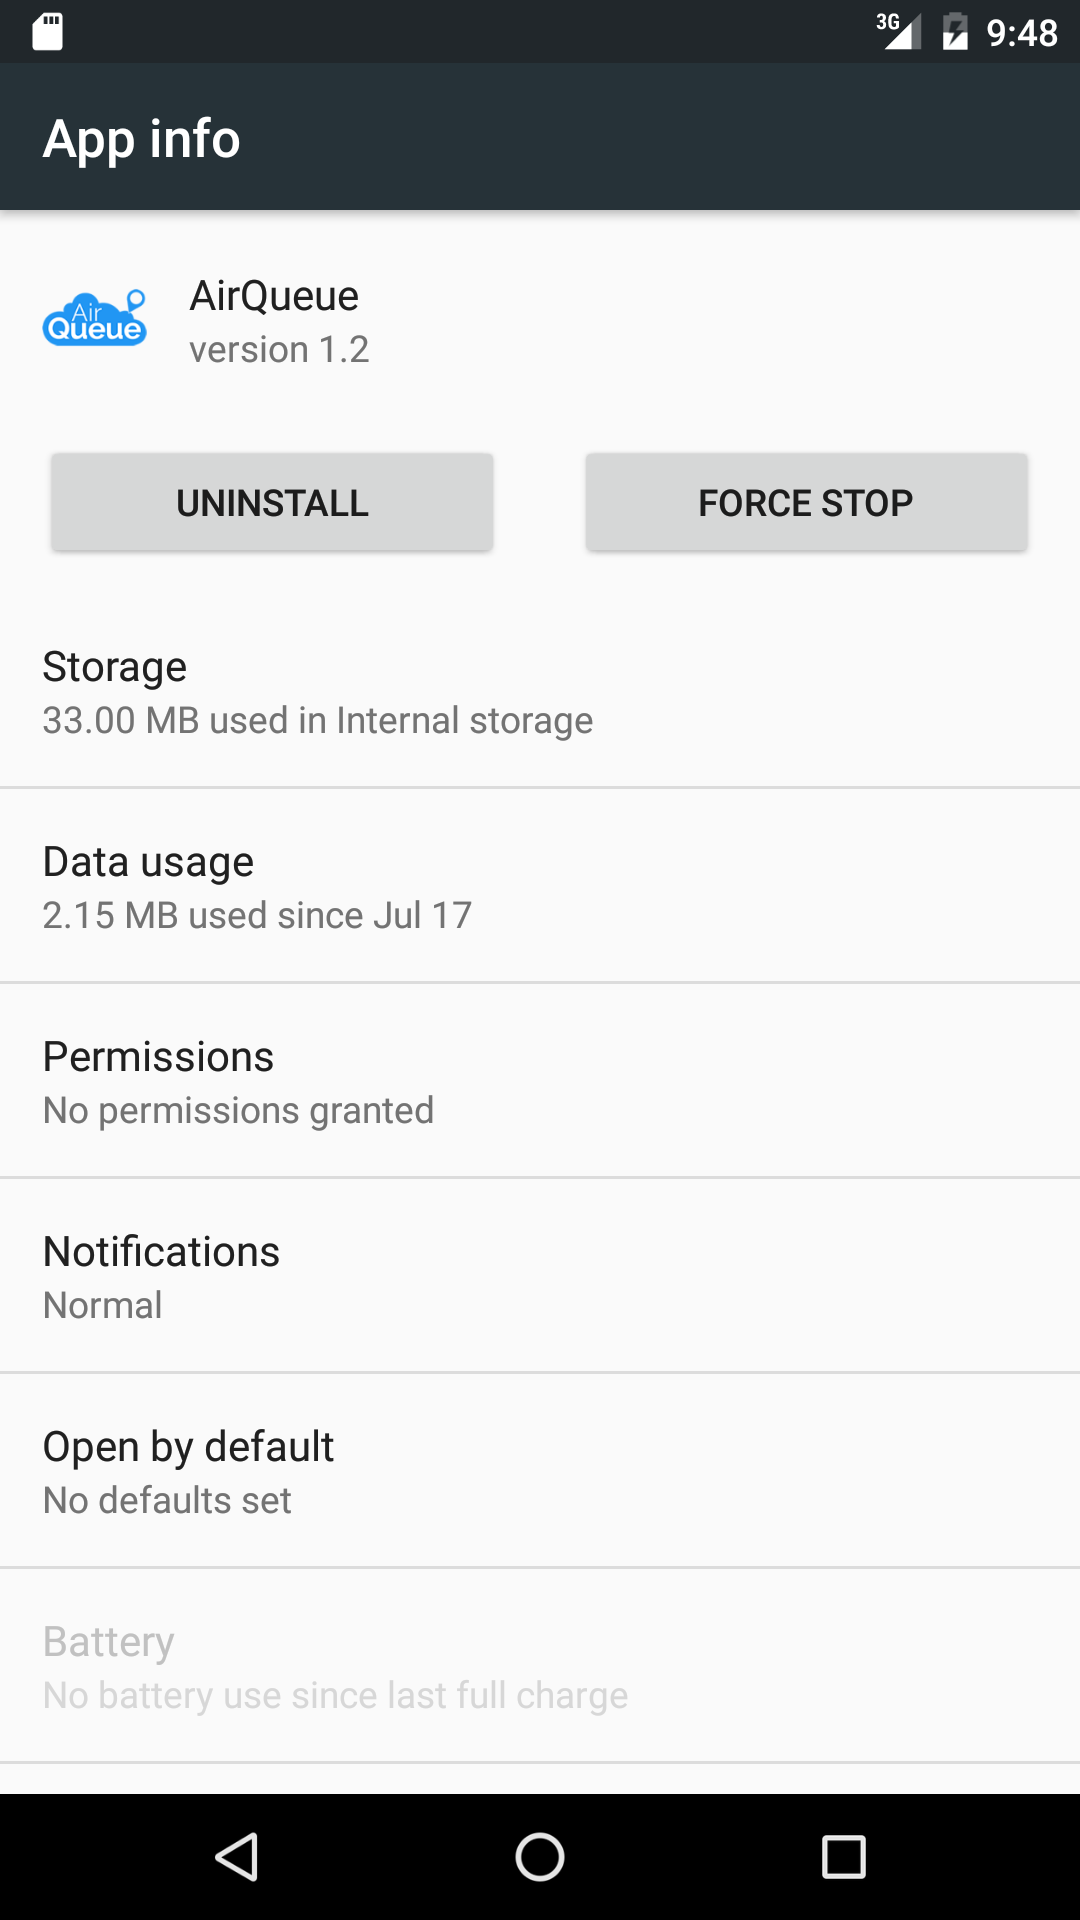
\includegraphics[scale=1]{images/resource_usage.png}
\end{adjustbox}
  \caption[Application resource usage]{Application resource usage}
  \label{fig:automated_tests}
\end{figure}


\section{Evaluation with Users}

The evaluation of a third prototype was carried out with potential final users of the application. That is, with volunteers from the AUKAR group, and from general users from the University of Edinburgh. The volunteers from AUKAR were potentially a good source of data because they were already aware of the issues around air quality and, therefore they would be motivated to give feedback. 
Two methods were employed for this purpose, a usability test complemented by a design critique. 

\subsection{Usability Testing}
To ensure the functional requirements as well as the usability attributes, it is helpful to test the product with real users under real-world circumstances. This outcome would provide more accurate feedback on how well users are interacting with the product in terms of the remaining selected attributes: usability and performance.

In total there were four participants, one from AUKAR, and three from the University of Edinburgh. All of them were new to the application. For the set-up, an Android phone (Motorola Moto G 3rd Gen.) was configured with the AirQueue app and a screen logger to observe the touches on the screen during the test. The room was equipped with a video recorder to keep log of what was said by the participants. P1, P2, P3 and P4 are the participants of the test. Their ages were 68, 28, 27 and 27 respectively. Their occupations are retired, designer, biologist and computer scientist. 

The test was divided into two parts in a one-hour individual meeting:

\begin{itemize}

	\item  The first part of the test consisted of executing small tasks or scenarios that should be accomplished within the interface, covering tasks in all visualisations and screens as shown in Table \ref{tab:test_scenarios}. Participants were asked to perform them individually and to indicate if they were able to do so with ease. Also, some of them were thinking aloud during the test. Each participant marked whether they were able to finish each of the tasks with ease as instructed with a n (No) or y (yes). 

The findings from this part of the test is that users were able to navigate the interface successfully using the visual and textual cues provided. Some of them were deviating from the instructions and discovering the interface on their own, suggesting that they were eager to explore elements that were calling their attention. Another finding is that tool-tips served a good guiding function as most of the participants used them to better understand the navigation through the interface.

	\item The second part of the usability test was guided by a usability scale inspired by Brooke's scale \cite{Brooke1996}. The users were asked to evaluate their experience ranking their agreement over different statements (1 strongly disagree, and 5 strongly agree). The employed usability scale and the responses are shown in Table \ref{tab:test_usability_scale}. 


From this part of the test it was confirmed that the overall satisfaction of the inter-face was good. The users felt that the interface displayed quick and smooth behavior that allowed them navigate with ease the different screens. Another interesting outcome is that the simple colour and textual indicators (good/regular/bad and green/yellow/red) helped the users to understand the air quality status, suggesting they might be a good instrument to disseminate data in a quick and understandable way. The main outcome is that the respondents stated they would use the application to know more about pollution in general and that its usage would help them to make better choices, suggesting that AirQueue could bring behavioural change and that it usage could be a good fit in their lives.

\end{itemize}




\iffalse
\begin{figure}[H]
\begin{adjustbox}{width=.8\textwidth,center=\textwidth}
  \centering
  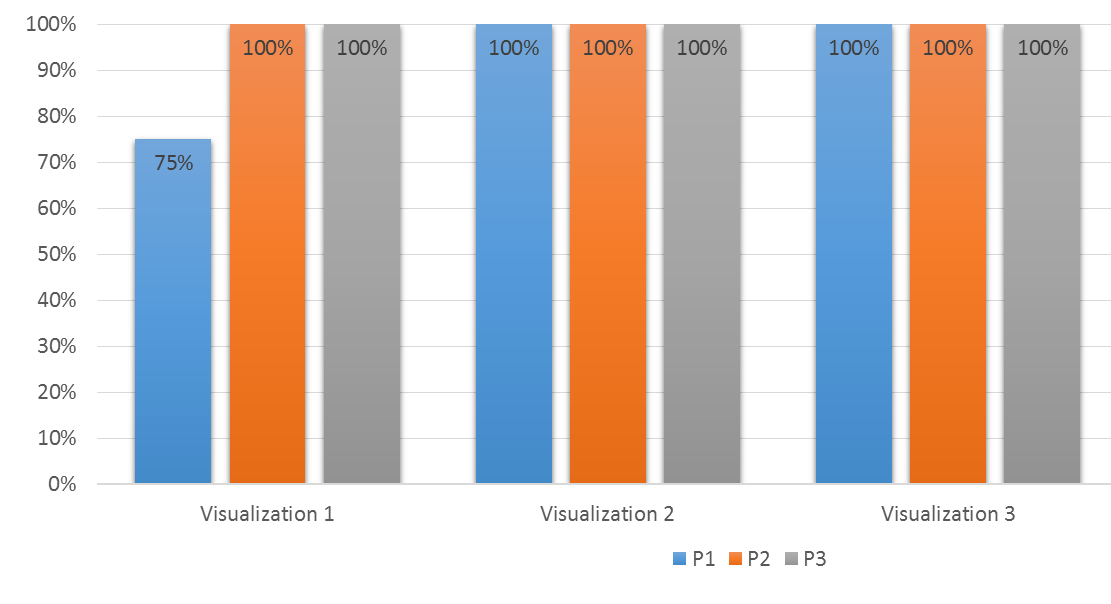
\includegraphics[scale=1]{images/scenarios_rate.png}
\end{adjustbox}
  \caption[Scenario tests completion rate]{Scenario tests completion rate}
  \label{fig:automated_tests}
\end{figure}
\fi

\newcommand{\specialcell}[2][c]{%
  \begin{tabular}[#1]{@{}l@{}}#2\end{tabular}}

\begin{table}[H]
\centering
\begin{adjustbox}{width=1\textwidth,center=\textwidth}
\begin{tabular}{llrrrr}
  \hline
   Tab/Screen & Activity & P1 & P2 & P3 & P4\\ \hline
   Overview & \specialcell[t]{1.-I want to start the application and reach the first\\'overview' screen.}  & y & y & y & y \\
   Overview & \specialcell[t]{2.-I want to visualise the location of the closest air\\quality-sensor and know when was it last updated..} & y & y & y & y \\
   Overview & \specialcell[t]{3.-I want to adjust my sensitivity level to indicate I have\\high sensitivity.} & y & y & y & y \\
   Overview & \specialcell[t]{4.-I want to know the air quality index. (How good or bad\\the air quality is).} & y & y & y & y \\
   Overview & \specialcell[t]{5.-I want to read my personalised health advice.\\} & y & y & y & y \\
   Overview &\specialcell[t]{6.-I want to adjust again my sensitivity level to indicate I\\have a low sensitivity and read my advice again.} & y & y & y & y \\
   Pollutants &\specialcell[t]{7.-I want to navigate to the second 'Pollutants' screen.} & y & y & y & y \\
   Pollutants &\specialcell[t]{8.-I want to examine the measured value for the sulphur\\dioxide pollutant.} & n & y & y & y \\
   Pollutants &\specialcell[t]{9.-I want to know if the measured value for sulphur\\dioxide is categorised as good, regular, bad or extremely\\bad.} & y & y & y & y \\
   Pollutants &\specialcell[t]{10.-I want to know further information about particulate\\matter. I want to read the sources and health effects of\\
   this specific pollutant.} & y & y & y & y \\
   Graphs &\specialcell[t]{11.-I want to navigate to the third 'Graphs' screen.} & y & y & y & y \\
   Graphs &\specialcell[t]{13.-I want to select the 'CO' pollutant and visualise the\\measured values through the day.} & y & y & y & y \\
   Graphs &\specialcell[t]{14.-I want to select the PM10 pollutant and visualise the\\measured values for yesterday.} & y & y & y & y \\
   \hline
\end{tabular}
\end{adjustbox}
  \caption[Usability testing scenarios]{Usability testing scenarios and results}
\label{tab:test_scenarios}
\end{table} 



\begin{table}[H]
\centering
\begin{adjustbox}{width=1.2\textwidth,center=\textwidth}
\begin{tabular}{llrrrr}
  \hline
   - & Statement & P1 & P2 & P3 & P4 \\ \hline
   Overview & \specialcell[t]{1.-I think that the first screen (overview) was easy to\\understand/navigate.} & 3 & 5 & 4  & 5 \\
   Overview &\specialcell[t]{2.- I think that the 'overview' screen would help me to understand the\\current situation of air quality.} & 5 & 4 & 5 & 5 \\
   Overview &\specialcell[t]{3.- I think that the personalised health 'advice' would help me to take better\\choices through the day.} & 5 & 4 & 5 &4 \\
   Overview &\specialcell[t]{4.- I feel that is useful to know the location of the closest air quality sensor.} & 5 & 5 & 4 & 4 \\
   Overview &\specialcell[t]{5.- I think that the colours of the 'overview' screen help me to\\understand the usage of the screen components.} & 1 & 5 & 4 &5 \\
   Overview &\specialcell[t]{6.- In the 'overview' screen, I think that the wording of the menus, labels and\\pop-ups is clear and concise.} & 3 & 5 & 5 &4 \\
   Pollutants &\specialcell[t]{7.- I think that the second screen (pollutants) was easy to\\understand/navigate.} & 5 & 5 & 5 &5 \\
   Pollutants &\specialcell[t]{8.- The 'pollutants' screen would help me to understand the current situation of air\\quality.} & 5 & 5 & 5 &5 \\   
   Pollutants &\specialcell[t]{9.- In the 'pollutants' screen the individual pollutant circles help me to understand\\easily how good or bad the measurements are. } & 5 & 5 & 5 &5 \\   
   Pollutants &\specialcell[t]{10.- It is useful to have information about the sources and effects of air pollution. } & 5 & 4 & 4 &5 \\   
   Graphs &\specialcell[t]{11.- I think that the third screen (graphs) was easy to understand/navigate.} & 5 & 5 & 5 &5 \\   
   Graphs &\specialcell[t]{12.- I think that the third screen 'Graphs' would be useful to track my response to\\certain pollutants.} & 5 & 5 & 5 &4 \\   
   Graphs &\specialcell[t]{13.- In the graphs screen the pollutant different colours help me to differentiate them.} & 5 & 5 & 4 &5 \\   
   Graphs &\specialcell[t]{14.- In the third screen (Graphs) the pollutant graphs are displayed promptly.} & 5 & 5 & 5 &5 \\   
   App in general &\specialcell[t]{15.- I think that it was easy to access and navigate through all the three screens.} & 4 & 5 & 5 &5 \\     
   App in general &\specialcell[t]{16.- I would imagine that most people would learn to use this system very quickly.} & 4 & 5 & 5 &4 \\ 
   App in general &\specialcell[t]{17.- I needed to learn a lot of things before I could get going with this system.} & 5 & 1 & 1 &1 \\ 
   App in general &\specialcell[t]{18.- I would say that the colours of the application help me to understand it better.} & 5 & 5 & 5 &4 \\ 
   App in general &\specialcell[t]{19.- I think that the application response to my actions wast fast and smooth.} & 5 & 5 & 5 &5 \\    
   App in general &\specialcell[t]{20.- The application starts promptly } & 5 & 5 & 5 &5 \\       
   App in general &\specialcell[t]{21.- I thought that simple indicators such as 'good', 'regular', 'bad' helped to understand\\the current air quality status.} & 5 & 5 & 5 &5 \\       
   App in general &\specialcell[t]{22.- I thought that colour indicators (green/yellow/red) helped to understand the\\current air quality status.} & 5 & 5 & 5 &5 \\          
   App in general &\specialcell[t]{23.- I would use this application to make better choices about my health.} & 5 & 5 & 5 &4 \\             
   App in general &\specialcell[t]{24.- I would use this application to know more about pollution in general.} & 5 & 4 & 4 &5 \\                
   App in general &\specialcell[t]{25.- I think using this application is fun and enjoyable.} & 3 & 4 & 4 & 4 \\         
   App in general &\specialcell[t]{26.- Having an 'smart' health advice   would help making my life easier.} & 5 & 5 & 5 &5 \\      
   App in general &\specialcell[t]{27.- It is more engaging or interesting using an application instead of a website to get\\information about pollution} & 5 & 4 & 5 & 5 \\         
   \hline
\end{tabular}
\end{adjustbox}
  \caption[Usability testing scale]{Usability testing scale and results.}
\label{tab:test_usability_scale}
\end{table} 

\subsection{Design Critique}
At the end of the meeting, participants were asked to give their thoughts on the application. This was an open discussion where the participants were guided through a couple of questions to find out more about what they liked, disliked, found useful or would add to the application. 

\bigskip
\textbf{What do you think about the interface?}
\bigskip

\begin{itemize}
	\item \quotes{The interface is very clean.}
    \item \quotes{It looks nice.}
    \item \quotes{This is almost like the front page on a book isn't it?} - Referring to the first screen.
\iffalse    \item \quotes{I didn't realize how to move away this tool-tip.} \fi
\end{itemize}

\bigskip
\textbf{Do you think having an application like this would help you to stay more informed about air pollution?}
\bigskip

\begin{itemize}
	\item \quotes{It would, because that way I can decide what to do based on what I see.}
    \item \quotes{Yes I think it would be as it would potentially mean I could change what I am doing that day to protect myself.}
\end{itemize}

\bigskip
\textbf{If you could add something, what would it be?}
\bigskip

\begin{itemize}
	\item \quotes{I was expecting this to react, it didn't occur to me that it was an introduction.} - Referring to the live pollutants section on the Overview screen. 
\end{itemize}

\bigskip
\textbf{What do you like about the application?}
\bigskip

\begin{itemize}
	\item \quotes{I like the way you can adjust, presumably once you've adjusted it, everything else in the screen takes it into account.} - Referring the personalised health advice.
\end{itemize}

\subsection{Summary}
The outcomes from the components of the test with users were positive. All participants were able to use the application in a confident way and believed that the application would make their lives easier. As a remark, it should be noted the relation between the ages of the participants and their outcome on both parts of the test. While P2, P3 and P4 where able to understand the scenarios whit ease and independently, P1 struggled on one task. Furthermore, P1 believed that some screens were slightly more difficult to use and that he would need to learn before using the app. Thus, P1 is an important representative user because those from an older generation are at less ease with smart phone apps.